
%% bare_conf.tex
%% V1.3
%% 2007/01/11
%% by Michael Shell
%% See:
%% http://www.michaelshell.org/
%% for current contact information.
%%
%% This is a skeleton file demonstrating the use of IEEEtran.cls
%% (requires IEEEtran.cls version 1.7 or later) with an IEEE conference paper.
%%
%% Support sites:
%% http://www.michaelshell.org/tex/ieeetran/
%% http://www.ctan.org/tex-archive/macros/latex/contrib/IEEEtran/
%% and
%% http://www.ieee.org/

%%*************************************************************************
%% Legal Notice:
%% This code is offered as-is without any warranty either expressed or
%% implied; without even the implied warranty of MERCHANTABILITY or
%% FITNESS FOR A PARTICULAR PURPOSE! 
%% User assumes all risk.
%% In no event shall IEEE or any contributor to this code be liable for
%% any damages or losses, including, but not limited to, incidental,
%% consequential, or any other damages, resulting from the use or misuse
%% of any information contained here.
%%
%% All comments are the opinions of their respective authors and are not
%% necessarily endorsed by the IEEE.
%%
%% This work is distributed under the LaTeX Project Public License (LPPL)
%% ( http://www.latex-project.org/ ) version 1.3, and may be freely used,
%% distributed and modified. A copy of the LPPL, version 1.3, is included
%% in the base LaTeX documentation of all distributions of LaTeX released
%% 2003/12/01 or later.
%% Retain all contribution notices and credits.
%% ** Modified files should be clearly indicated as such, including  **
%% ** renaming them and changing author support contact information. **
%%
%% File list of work: IEEEtran.cls, IEEEtran_HOWTO.pdf, bare_adv.tex,
%%                    bare_conf.tex, bare_jrnl.tex, bare_jrnl_compsoc.tex
%%*************************************************************************

% *** Authors should verify (and, if needed, correct) their LaTeX system  ***
% *** with the testflow diagnostic prior to trusting their LaTeX platform ***
% *** with production work. IEEE's font choices can trigger bugs that do  ***
% *** not appear when using other class files.                            ***
% The testflow support page is at:
% http://www.michaelshell.org/tex/testflow/



% Note that the a4paper option is mainly intended so that authors in
% countries using A4 can easily print to A4 and see how their papers will
% look in print - the typesetting of the document will not typically be
% affected with changes in paper size (but the bottom and side margins will).
% Use the testflow package mentioned above to verify correct handling of
% both paper sizes by the user's LaTeX system.
%
% Also note that the "draftcls" or "draftclsnofoot", not "draft", option
% should be used if it is desired that the figures are to be displayed in
% draft mode.
%
\documentclass[conference]{IEEEtran}
% Add the compsoc option for Computer Society conferences.
%
% If IEEEtran.cls has not been installed into the LaTeX system files,
% manually specify the path to it like:
% \documentclass[conference]{../sty/IEEEtran}





% Some very useful LaTeX packages include:
% (uncomment the ones you want to load)


% *** MISC UTILITY PACKAGES ***
%
%\usepackage{ifpdf}
% Heiko Oberdiek's ifpdf.sty is very useful if you need conditional
% compilation based on whether the output is pdf or dvi.
% usage:
% \ifpdf
%   % pdf code
% \else
%   % dvi code
% \fi
% The latest version of ifpdf.sty can be obtained from:
% http://www.ctan.org/tex-archive/macros/latex/contrib/oberdiek/
% Also, note that IEEEtran.cls V1.7 and later provides a builtin
% \ifCLASSINFOpdf conditional that works the same way.
% When switching from latex to pdflatex and vice-versa, the compiler may
% have to be run twice to clear warning/error messages.

% *** CITATION PACKAGES ***
%
\usepackage{cite}
% cite.sty was written by Donald Arseneau
% V1.6 and later of IEEEtran pre-defines the format of the cite.sty package
% \cite{} output to follow that of IEEE. Loading the cite package will
% result in citation numbers being automatically sorted and properly
% "compressed/ranged". e.g., [1], [9], [2], [7], [5], [6] without using
% cite.sty will become [1], [2], [5]--[7], [9] using cite.sty. cite.sty's
% \cite will automatically add leading space, if needed. Use cite.sty's
% noadjust option (cite.sty V3.8 and later) if you want to turn this off.
% cite.sty is already installed on most LaTeX systems. Be sure and use
% version 4.0 (2003-05-27) and later if using hyperref.sty. cite.sty does
% not currently provide for hyperlinked citations.
% The latest version can be obtained at:
% http://www.ctan.org/tex-archive/macros/latex/contrib/cite/
% The documentation is contained in the cite.sty file itself.


\usepackage[utf8]{inputenc}


% *** GRAPHICS RELATED PACKAGES ***
%
\ifCLASSINFOpdf
  \usepackage[pdftex]{graphicx}
  % declare the path(s) where your graphic files are
  % \graphicspath{{../pdf/}{../jpeg/}}
  % and their extensions so you won't have to specify these with
  % every instance of \includegraphics
  % \DeclareGraphicsExtensions{.pdf,.jpeg,.png}
\else
  % or other class option (dvipsone, dvipdf, if not using dvips). graphicx
  % will default to the driver specified in the system graphics.cfg if no
  % driver is specified.
  % \usepackage[dvips]{graphicx}
  % declare the path(s) where your graphic files are
  % \graphicspath{{../eps/}}
  % and their extensions so you won't have to specify these with
  % every instance of \includegraphics
  % \DeclareGraphicsExtensions{.eps}
\fi
% graphicx was written by David Carlisle and Sebastian Rahtz. It is
% required if you want graphics, photos, etc. graphicx.sty is already
% installed on most LaTeX systems. The latest version and documentation can
% be obtained at: 
% http://www.ctan.org/tex-archive/macros/latex/required/graphics/
% Another good source of documentation is "Using Imported Graphics in
% LaTeX2e" by Keith Reckdahl which can be found as epslatex.ps or
% epslatex.pdf at: http://www.ctan.org/tex-archive/info/
%
% latex, and pdflatex in dvi mode, support graphics in encapsulated
% postscript (.eps) format. pdflatex in pdf mode supports graphics
% in .pdf, .jpeg, .png and .mps (metapost) formats. Users should ensure
% that all non-photo figures use a vector format (.eps, .pdf, .mps) and
% not a bitmapped formats (.jpeg, .png). IEEE frowns on bitmapped formats
% which can result in "jaggedy"/blurry rendering of lines and letters as
% well as large increases in file sizes.
%
% You can find documentation about the pdfTeX application at:
% http://www.tug.org/applications/pdftex





% *** MATH PACKAGES ***
%
%\usepackage[cmex10]{amsmath}
% A popular package from the American Mathematical Society that provides
% many useful and powerful commands for dealing with mathematics. If using
% it, be sure to load this package with the cmex10 option to ensure that
% only type 1 fonts will utilized at all point sizes. Without this option,
% it is possible that some math symbols, particularly those within
% footnotes, will be rendered in bitmap form which will result in a
% document that can not be IEEE Xplore compliant!
%
% Also, note that the amsmath package sets \interdisplaylinepenalty to 10000
% thus preventing page breaks from occurring within multiline equations. Use:
%\interdisplaylinepenalty=2500
% after loading amsmath to restore such page breaks as IEEEtran.cls normally
% does. amsmath.sty is already installed on most LaTeX systems. The latest
% version and documentation can be obtained at:
% http://www.ctan.org/tex-archive/macros/latex/required/amslatex/math/





% *** SPECIALIZED LIST PACKAGES ***
%
%\usepackage{algorithmic}
% algorithmic.sty was written by Peter Williams and Rogerio Brito.
% This package provides an algorithmic environment fo describing algorithms.
% You can use the algorithmic environment in-text or within a figure
% environment to provide for a floating algorithm. Do NOT use the algorithm
% floating environment provided by algorithm.sty (by the same authors) or
% algorithm2e.sty (by Christophe Fiorio) as IEEE does not use dedicated
% algorithm float types and packages that provide these will not provide
% correct IEEE style captions. The latest version and documentation of
% algorithmic.sty can be obtained at:
% http://www.ctan.org/tex-archive/macros/latex/contrib/algorithms/
% There is also a support site at:
% http://algorithms.berlios.de/index.html
% Also of interest may be the (relatively newer and more customizable)
% algorithmicx.sty package by Szasz Janos:
% http://www.ctan.org/tex-archive/macros/latex/contrib/algorithmicx/




% *** ALIGNMENT PACKAGES ***
%
%\usepackage{array}
% Frank Mittelbach's and David Carlisle's array.sty patches and improves
% the standard LaTeX2e array and tabular environments to provide better
% appearance and additional user controls. As the default LaTeX2e table
% generation code is lacking to the point of almost being broken with
% respect to the quality of the end results, all users are strongly
% advised to use an enhanced (at the very least that provided by array.sty)
% set of table tools. array.sty is already installed on most systems. The
% latest version and documentation can be obtained at:
% http://www.ctan.org/tex-archive/macros/latex/required/tools/


%\usepackage{mdwmath}
%\usepackage{mdwtab}
% Also highly recommended is Mark Wooding's extremely powerful MDW tools,
% especially mdwmath.sty and mdwtab.sty which are used to format equations
% and tables, respectively. The MDWtools set is already installed on most
% LaTeX systems. The lastest version and documentation is available at:
% http://www.ctan.org/tex-archive/macros/latex/contrib/mdwtools/


% IEEEtran contains the IEEEeqnarray family of commands that can be used to
% generate multiline equations as well as matrices, tables, etc., of high
% quality.


%\usepackage{eqparbox}
% Also of notable interest is Scott Pakin's eqparbox package for creating
% (automatically sized) equal width boxes - aka "natural width parboxes".
% Available at:
% http://www.ctan.org/tex-archive/macros/latex/contrib/eqparbox/





% *** SUBFIGURE PACKAGES ***
%\usepackage[tight,footnotesize]{subfigure}
% subfigure.sty was written by Steven Douglas Cochran. This package makes it
% easy to put subfigures in your figures. e.g., "Figure 1a and 1b". For IEEE
% work, it is a good idea to load it with the tight package option to reduce
% the amount of white space around the subfigures. subfigure.sty is already
% installed on most LaTeX systems. The latest version and documentation can
% be obtained at:
% http://www.ctan.org/tex-archive/obsolete/macros/latex/contrib/subfigure/
% subfigure.sty has been superceeded by subfig.sty.



%\usepackage[caption=false]{caption}
%\usepackage[font=footnotesize]{subfig}
% subfig.sty, also written by Steven Douglas Cochran, is the modern
% replacement for subfigure.sty. However, subfig.sty requires and
% automatically loads Axel Sommerfeldt's caption.sty which will override
% IEEEtran.cls handling of captions and this will result in nonIEEE style
% figure/table captions. To prevent this problem, be sure and preload
% caption.sty with its "caption=false" package option. This is will preserve
% IEEEtran.cls handing of captions. Version 1.3 (2005/06/28) and later 
% (recommended due to many improvements over 1.2) of subfig.sty supports
% the caption=false option directly:
%\usepackage[caption=false,font=footnotesize]{subfig}
%
% The latest version and documentation can be obtained at:
% http://www.ctan.org/tex-archive/macros/latex/contrib/subfig/
% The latest version and documentation of caption.sty can be obtained at:
% http://www.ctan.org/tex-archive/macros/latex/contrib/caption/




% *** FLOAT PACKAGES ***
%
%\usepackage{fixltx2e}
% fixltx2e, the successor to the earlier fix2col.sty, was written by
% Frank Mittelbach and David Carlisle. This package corrects a few problems
% in the LaTeX2e kernel, the most notable of which is that in current
% LaTeX2e releases, the ordering of single and double column floats is not
% guaranteed to be preserved. Thus, an unpatched LaTeX2e can allow a
% single column figure to be placed prior to an earlier double column
% figure. The latest version and documentation can be found at:
% http://www.ctan.org/tex-archive/macros/latex/base/



%\usepackage{stfloats}
% stfloats.sty was written by Sigitas Tolusis. This package gives LaTeX2e
% the ability to do double column floats at the bottom of the page as well
% as the top. (e.g., "\begin{figure*}[!b]" is not normally possible in
% LaTeX2e). It also provides a command:
%\fnbelowfloat
% to enable the placement of footnotes below bottom floats (the standard
% LaTeX2e kernel puts them above bottom floats). This is an invasive package
% which rewrites many portions of the LaTeX2e float routines. It may not work
% with other packages that modify the LaTeX2e float routines. The latest
% version and documentation can be obtained at:
% http://www.ctan.org/tex-archive/macros/latex/contrib/sttools/
% Documentation is contained in the stfloats.sty comments as well as in the
% presfull.pdf file. Do not use the stfloats baselinefloat ability as IEEE
% does not allow \baselineskip to stretch. Authors submitting work to the
% IEEE should note that IEEE rarely uses double column equations and
% that authors should try to avoid such use. Do not be tempted to use the
% cuted.sty or midfloat.sty packages (also by Sigitas Tolusis) as IEEE does
% not format its papers in such ways.





% *** PDF, URL AND HYPERLINK PACKAGES ***
%
%\usepackage{url}
% url.sty was written by Donald Arseneau. It provides better support for
% handling and breaking URLs. url.sty is already installed on most LaTeX
% systems. The latest version can be obtained at:
% http://www.ctan.org/tex-archive/macros/latex/contrib/misc/
% Read the url.sty source comments for usage information. Basically,
% \url{my_url_here}.


%%% Custom Packages %%%
\usepackage{flushend}


% *** Do not adjust lengths that control margins, column widths, etc. ***
% *** Do not use packages that alter fonts (such as pslatex).         ***
% There should be no need to do such things with IEEEtran.cls V1.6 and later.
% (Unless specifically asked to do so by the journal or conference you plan
% to submit to, of course. )


% correct bad hyphenation here
\hyphenation{op-tical net-works semi-conduc-tor}


\begin{document}
%
% paper title
% can use linebreaks \\ within to get better formatting as desired
\title{True Random Generation on Mobile Phones}

% author names and affiliations
% use a multiple column layout for up to three different
% affiliations
\author{
\IEEEauthorblockN{Kevin Burns}
\IEEEauthorblockA{Department of Electrical and\\Computer Engineering\\
Virginia Tech\\
Blacksburg, Virginia\\
Email: kevinpb@vt.edu}
\and
\IEEEauthorblockN{Rob Lyerly}
\IEEEauthorblockA{Department of Electrical and\\Computer Engineering\\
Virginia Tech\\
Blacksburg, Virginia\\
Email: rlyerly@vt.edu}
\and
\IEEEauthorblockN{Reese Moore}
\IEEEauthorblockA{Department of Electrical and\\Computer Engineering\\
Virginia Tech\\
Blacksburg, Virginia\\
Email: ram@vt.edu}
\and
\IEEEauthorblockN{Philip Kobezak}
\IEEEauthorblockA{Department of Electrical and\\Computer Engineering\\
Virginia Tech\\
Blacksburg, Virginia\\
Email: pkobezak@vt.edu}
}

% conference papers do not typically use \thanks and this command
% is locked out in conference mode. If really needed, such as for
% the acknowledgment of grants, issue a \IEEEoverridecommandlockouts
% after \documentclass

% for over three affiliations, or if they all won't fit within the width
% of the page, use this alternative format:
% 
%\author{\IEEEauthorblockN{Michael Shell\IEEEauthorrefmark{1},
%Homer Simpson\IEEEauthorrefmark{2},
%James Kirk\IEEEauthorrefmark{3}, 
%Montgomery Scott\IEEEauthorrefmark{3} and
%Eldon Tyrell\IEEEauthorrefmark{4}}
%\IEEEauthorblockA{\IEEEauthorrefmark{1}School of Electrical and Computer Engineering\\
%Georgia Institute of Technology,
%Atlanta, Georgia 30332--0250\\ Email: see http://www.michaelshell.org/contact.html}
%\IEEEauthorblockA{\IEEEauthorrefmark{2}Twentieth Century Fox, Springfield, USA\\
%Email: homer@thesimpsons.com}
%\IEEEauthorblockA{\IEEEauthorrefmark{3}Starfleet Academy, San Francisco, California 96678-2391\\
%Telephone: (800) 555--1212, Fax: (888) 555--1212}
%\IEEEauthorblockA{\IEEEauthorrefmark{4}Tyrell Inc., 123 Replicant Street, Los Angeles, California 90210--4321}}

% use for special paper notices
%\IEEEspecialpapernotice{(Invited Paper)}

% make the title area
\maketitle

\begin{abstract}
%\boldmath
    With mobile platforms becoming more ubiquitous in modern society there is a greater need for the ability to run cryptographic algorithms on 
    low power architectures, most of which require a source of randomness. For the Android version of the Linux kernel this randomness is provided
    by user input and timing data. However, these few sources of entropy have proven to be very slow and many implementations choose to forego good
    random numbers and use highly deterministic replacements in their stead. Therefore there is a high demand for a quick and power efficient
    random number generator for embedded and mobile devices.  We evaluate two potential sources common on most Android devices, the gyroscope and
    accelerometer, as sources of true random numbers.  We show that significant work is required to make the data obtained from these sources
    usable for true random number generation.
\end{abstract}

% IEEEtran.cls defaults to using nonbold math in the Abstract.
% This preserves the distinction between vectors and scalars. However,
% if the conference you are submitting to favors bold math in the abstract,
% then you can use LaTeX's standard command \boldmath at the very start
% of the abstract to achieve this. Many IEEE journals/conferences frown on
% math in the abstract anyway.

% no keywords

% For peer review papers, you can put extra information on the cover
% page as needed:
% \ifCLASSOPTIONpeerreview
% \begin{center} \bfseries EDICS Category: 3-BBND \end{center}
% \fi
%
% For peerreview papers, this IEEEtran command inserts a page break and
% creates the second title. It will be ignored for other modes.
\IEEEpeerreviewmaketitle

\section{Introduction}
At the core of the majority cryptography operations, there exists a need for true random numbers. 
High-end true random number generators (TRNGs) can be costly to produce and are power-intensive; the fastest known TRNG was produced
in 2010 at Bar-Ilan University \cite{kanter}, which claimed to generate data at a rate of $300 Gbit/s$ using a derivative
of digitized chaotic laser intensity. However, many traditional approaches to hardware random number generation are not suitable in a
mobile or embedded environment, as access to such high-power noisy devices is simply not feasible. Nevertheless, the need for such
random number generators is rising as many types of applications which require cryptographically secure communication (e-mail, banking,
transfer of secure data) are being pushed into the mobile phone realm.  Previous research suggests that current mobile and embedded
devices opt for quick and easy replacements for TRNGs that cause severe security vulnerabilities in sensitive contexts \cite{chip_and_skim}.
Because of this, there is a strong need for fast, high quality TRNGs on mobile and embedded platforms.  As prior work suggests that
sensors common to many embedded systems are good sources of highly entropic random data, we investigate a practical approach to
construction of a TRNG suitable for currently deployed (as well as future) Android devices.

\subsection{Background}
%Linux Entropy Pool
The Linux kernel, used as the basis for Android, has an entropy pool to provide data to applications that require truly random bits.
This pool is populated via environmental noise from device drivers, timing differences between interrupts, and other various
sources. These sources are viewed as true random number generators and therefore provide entropy suitable for key generation and other
cryptography. Access to this pool is granted through the random device located at /dev/random \cite{random_man} and through the urandom device, 
located at /dev/urandom. These two interfaces read from the entropy pool until a limit of 128 bits of remaining entropy is reached. Once
the pool is drained below this bit limit, the two devices behave differently.  If the application reading from the pool is using the random
interface, the application will block until more entropy is added to the pool. Alternatively, the urandom interface provides ``unlimited''
entropy by rehashing existing entropy in the pool. The urandom device does not block, but forgoes true randomness and feeds pseudo random
data to the application. The pseudo-random nature of this device means that it is theoretically vulnerable to cryptographic attacks.

%Seeder
Developers have created an app available in the Google Play Store entitled Seeder, which attempts to cope with the blocking nature of the random
device by ensuring that entropic bits are always available.  Their solution to provide entropy even when the random device's 128 bit limit is
reached is to pipe pseudo-random data from the urandom device back into the entropy pool. The developers of Seeder claim this provides noticeable
speedups in day to day use of the Android operating system; however, this theoretically creates a security hole by reducing the true randomness of
random to a pseudo-random level. As this application has been downloaded over ten thousand times in the past 30 days (as of the date this paper
was written), it is clear that this is an area of interest to the Android user community.

\section{Related Work}
%The Sources of Randomness in Mobile Devices
The task of finding true randomness on mobile platforms has been targeted before. In \cite{Krhovjak}, the two main sources analyzed were the 
camera and microphone. The authors of this paper were unable to generate definite bit-rates for random number generation but were able to verify
the validity of the data generated.  There were several advantages and disadvantages presented in this paper in regards to the camera as a random
number generator. The advantages included the ability to produce considerable entropy even at low temperatures and when the camera guard was
closed. However there were also some vulnerabilities; an attacker could use a halogen light bulb to saturate the Charge-Coupled
Device (CCD), producing values of 255 for the R, G, and B values of each pixel, highly biasing the randomness produced by the camera. 
The microphone's noise as a source of randomness was found to be 3 bits of entropy per sample given by the Shannon entropy formula and 0.5 using the
min-entropy formula. The only attempt to skew the data was by playing two sets of recordings - one recording of music and one with ambient background
noises. They did find correlations between randomness generated from the music recording, but stated that this could be corrected with the proper
post-processing.  They also mentioned that manufacturers of both microphones and cameras are continuously trying to decrease the noise in their devices
via both hardware and proprietary (hidden) software. The tests mentioned in \cite{Krhovjak} were performed in 2007 on dated hardware, meaning newer
models of these cameras and microphones may not be as suitable as sources of random numbers.

% Touchscreens as a source of randomness
%touchscreen

Additional research has also explored the use of a mobile device's touch 
screen as a source for random number generation.  One particular paper 
\cite{montville2003random}, discussed the use of an input application presented 
to the end-user where they would move their finger to generate 
coordinates.  These coordinates were filtered to only use the lower 
eight bits of each value and produced good entropy.  However, this 
solution is only good for generating random data infrequently.  An 
example use might be generating a password or key that doesn't change
frequently.  For encrypting session data, such as TLS, it would require
more interaction from the end-user and be inconvenient.


%Accelerometers and Randomness: Perfect Together
Accelerometers have also been studied as a potential source of entropy in low-power and embedded devices.  J. Voris et al. analyzed the use of
accelerometers in an Intel WISP RFID tag \cite{voris}.  They conclude that even when stationary, accelerometers are sensitive enough to provide
a good rate of entropy (they test the device when at rest on industrial dampening material).  They show that accelerometers are
highly resistant to bias, arguing that the best attack vector to reduce randomness is to leave the accelerometer stationary; in other words,
movement only serves to increase the level randomness rather than degrade it.  While it is conceivable that an attacker could saturate the device's
output by applying an extraordinary force (say, in a centrifuge), an accelerometer lacks the potential for bias that plagues many of the other
devices on the phone.  Although gyroscopes have not been studied as a means for random number generation, they are similar to accelerometers in
that they strive to achieve a high level of sensitivity.  In addition, these two devices have become ubiquitous on modern phones and are extremely
cheap to include in any system.  Because of the low potential for bias mentioned in \cite{voris} and the widespread inclusion of these devices,
they are an attractive means for adding entropy to a random number generator.

%old
%\subsection{Problem Statement}
%Due to the increasing number of mobile platforms and their use of cryptographic algorithms and random number generators, there is demand for quick 
%and power efficient random number generators in the mobile environment. Specifically on our target hardware, Qualcomm's APQ8060 Dragonboard, we have 
%access to the random and urandom devices given via the Linux kernel. The random device is the true random number generation option in the Linux 
%environment, it is therefore a safe baseline for comparison as it is fairly consistent between Android devices. There are issues with this current solution.
%Firstly, a performance decrease can be witnessed when the entropy pool, used by random, is depleted to 128 bits. This is may be more prevalent in Android's
%Event Loop software model, as there isn't a clear multi-tasking structure. Another flaw comes to the scene when programmers and users try to circumvent
%this performance drain, by either filling the entropy pool with a none random bit-stream or by using the urandom device where the random device is more secure.
%We witness the effects of these issues in sources like \cite{ron_was_wrong}, which found that 4\% of 6.6 million certificates and PGP keys use the same RSA 
%modulus and therefore possibly have the exact same private key as someone else. The authors of \cite{chip_and_skim} exposed poor random number generators
%in EMV machines, used in chip and pin payments. Companies, such as Qualcomm, provide hardware random number generators in their System on a Chip (SoC) architectures to combat these drawbacks. 
%Therefore there is a clear need for a low power solution that is applicable to existing and future mobile devices on the market.

%new
\subsection{Problem Statement}
Due to the increasing number of mobile platforms and their use of cryptographic algorithms and random number generators, there is demand for quick 
and power efficient random number generators in the mobile environment. Specifically we targeted Android based smart phones,this grants us 
access to the random and urandom devices given via the Linux kernel. The random device is the true random number generating option in the Linux 
environment, it is therefore a safe baseline for comparison as it is fairly consistent between Android devices. There are several issues with this current solution.
Firstly, a performance decrease can be witnessed when the entropy pool, used by the random device, is depleted to 128 bits. This may be more prevalent in Android's
Event Loop software model, as there isn't a clear multi-tasking structure. Another flaw comes to the scene when programmers and users try to circumvent
this performance drain, by either filling the entropy pool with a none random bit-stream or by using the urandom device when the random device is more secure.
We witness the effects of these issues in sources like \cite{ron_was_wrong}, which found that 4\% of 6.6 million certificates and PGP keys use the same RSA 
modulus and therefore possibly have the exact same private key as someone else. The authors of \cite{chip_and_skim} exposed poor random number generators
in EMV machines, used in chip and pin payments. Companies, such as Qualcomm, provide hardware random number generators in their System on a Chip (SoC) architectures to combat these drawbacks. 
Therefore there is a clear need for a low power true random generator that is applicable to legacy and future mobile devices on the market.

\section{Proposed Solution}
%Kevin: possibly change to have independent post processing blocks and change the word daemon
\begin{figure}[t]
	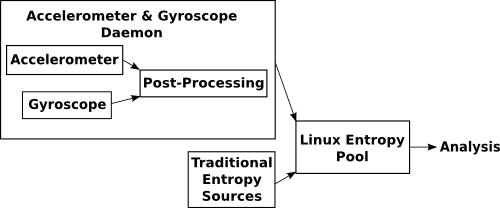
\includegraphics[width=\columnwidth]{proposed_solution}
	\caption{Block diagram of the proposed solution.  Our application will poll from the accelerometer and gyroscope (when requested), perform post-processing and feed random bits into the Linux entropy pool via system calls.}
	\label{proposed_solution_block}
\end{figure}
Although mobile phones have many different devices on-chip that could be
potentially used as sources of randomness for a random number generator, most of
these devices have the potential for strong bias.  Additionally, because of the
operating environment, polling these devices with high frequency can cause
serious system performance and energy issues.  Therefore, it is necessary to not
only use devices that have high quality randomness, but to use those devices in
an intelligent manner so as to not overwhelm the computational and energy
resources of the device.

We propose the implementation of a Android process that polls data from the
accelerometer and gyroscope (when the entropy pool is running low), processes
input data to eliminate sources of bias, and feeds the data into the entropy
pool.  Fig.~\ref{proposed_solution_block} shows the architecture for our
application. Android built on Linux exposes standard interfaces to the hardware
sensors for data retrieval; additionally, Linux provides system calls to feed
random data into the entropy pool.  Our application will interact with both of
these interfaces.

%There are many types of post processing that can be implemented to increase the
%uniformity of the random numbers generated.  Hash algorithms like SHA-3
%\cite{keccak} can be used to eliminate bias.  Similarly, Barak et al. propose a
%technique whereby random numbers are pulled from several independent devices
%\cite{independent_devices}.  Two of these numbers are multiplied together and
%added to a third number to strengthen the randomness.  Barak et al. propose
%another technique where random numbers are multiplied by a Toeplitz matrix to
%approach a uniform distribution \cite{true_rng}.  These techniques will be
%implemented and compared for their effectiveness and computational complexity.
%
%Random numbers generated by our daemon will be compared to the stock
%Android/Linux random number generator (which includes an on-board hardware RNG
%that may not be present on all mobile devices).  These two sources will be
%compared on three dimensions: quality of random numbers generated, energy draw
%from using the random number generator, and computational resources used by
%random number generation.  The DIEHARD \cite{diehard} / NIST \cite{nist}
%benchmarks will be used to evaluate the quality of the random numbers
%generated; synthetic benchmarks will be written to evaluate the energy draw and
%computational complexity of the random number generators.

%just mention V. N. Whitening here?

%There are many types of post processing that can be implemented to increase the
%uniformity of the random numbers generated.  Hash algorithms like SHA-3
%\cite{keccak} can be used to eliminate bias.  Similarly, Barak et al. propose a
%technique whereby random numbers are pulled from several independent devices
%\cite{independent_devices}.  Two of these numbers are multiplied together and
%added to a third number to strengthen the randomness.  Barak et al. propose
%another technique where random numbers are multiplied by a Toeplitz matrix to
%approach a uniform distribution \cite{true_rng}.  These techniques will be
%implemented and compared for their effectiveness and computational complexity.

There are many types of post processing that can be implemented to increase the
uniformity of the random numbers generated. The post-processing proposed for the
scope of this paper is von Neumann Whitening \cite{vn_whitening} and basic bit
filtering. 

\begin{figure}
	\centering
	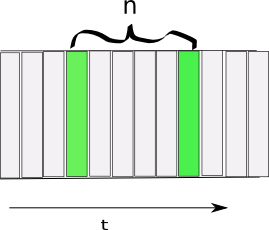
\includegraphics[width=0.25\textwidth]{vn_whitening.png}
	\caption{von Neumann whitening across several samples.}
	\label{fig:vnw}
\end{figure}

Von Neumann Whitening is a basic post processing procedure that takes two bits
at a time and processes them to give three possible outcomes. If the two bits
are the same, then they are simply discarded and there is no output. If the
sequence of bits is 0,1 then the output is 1 and conversely if the sequence of
bits is 1,0 then the output is 0. The rational behind this scheme is that it
will eliminate bias of the bits source towards a 1 or a 0. If the source is
biased towards either value with probability $p$, the probabilities for 1,0 and
0,1 are both equal to $p(1-p)$. With the same probability, they become a single
entropic bit. Unfortunately, this method only works to eliminate bias, but not
correlation between bits. The proposed solution attempts to reduce correlation
by using bits from samples taken $N$ samplings apart as can be seen in figure
\ref{fig:vnw} (in this case, $N = 1024$) and by using bit positions that are
offset from each other. 

The other method of improving the quality of the data that is pulled from the
sensors that is explored in this work is basic bit filtering. This is the simple
process of reading in all bits from the original source, and discarding those
that are suspected to be less random. Owing to the type of source that is being
polled, sensors, not all of the bits can be expected to be highly entropic or
even partially random. The data that can be retrieved from the Android sensor
API is returned as an IEEE 754 floating point number. As a result we can
immediately assume that both the sign bit and the exponent are unlikely to vary
much during normal use and are highly likely to be correlated between samplings.
Similarly, the most significant bits of the mantissa are intuitively more likely
to be correlated between samples than the least significant bit. The proposed
solution discards those bits that are suspected, through preimplementation
testing, of being of lesser quality randomness, though an ideal solution would
be able to sense the randomness of its incoming streams and filter accordingly
at runtime.



\subsection{Expectations}
%% Expectations

From the findings of \cite{voris}, accelerometers appear to be highly random. A
high rate of sampling shows that they are fairly fast and should be able to
provide a high rate of random bits per second when they are needed. The
specification sheet for the accelerometer found on the Dragonboard shows that it
is also efficient for power consumption.

The apparent randomness of the accelerometer and gyroscope, accompanied with the
relatively low power nature of the components as well as their ubiquity on smart
phones, tends to suggest that they would be an excellent source of entropy for
mobile platforms. A solution that pulls from these sensors should be easily
deployed to several different platforms, including those that do not have the
benefit of an on board hardware random number generator. As quality random
numbers are necessary for most of the common cryptographic operations, such a
system will be able to bring faster secure communication to more devices. 


\section{Experimental Setup}
%%%%%%%%%%%%%%%%%%%%%%%%%%%%%%%%%%%%%%%%%%%%%%%%%%%%%%%%%%%%%%%%%%%%%%%%%%%%%%%%
%% Experimental Setup:
%%  - What our methodology was
%%  - Details about the Phones
%%  - Some information about NIST
%%%%%%%%%%%%%%%%%%%%%%%%%%%%%%%%%%%%%%%%%%%%%%%%%%%%%%%%%%%%%%%%%%%%%%%%%%%%%%%%

In order to show that sampling accelerometer and gyroscope data is an effective
mechanism for randomness generation on mobile phones, a testing methodology was
developed. This testing methodology involved gathering data from mobile phones
and utilizing well regarded statistical analysis suites to determine the quality
of the results. To maintain data equivalence across testing, a single platform
was chosen for all of the tests. 

%%% Information about the Phone
%%%   - Specs
%%%   - Why it was chosen over other phones... lol
\subsection{Samsung Nexus S}

The platform used for testing was the Samsung Nexus S. The Nexus S was first
released in December of 2010. It uses a Samsung Exynos 3110 System on Chip
(SoC). The Exynos 3110 is a single core ARM Cortex-A8 using the ARMv7
instruction set. In the Nexus S, the processor operates at a 1GHz clock
frequency and is paired with 512MB of main memory. The phone originally shipped
with Android 2.3 installed but was updated to the latest supported build, 4.1.2.
The Nexus S has both a three-axis gyroscope and accelerometer provided by the
InvenSense MPU-6050. The MPU-6050 communicates to the CPU via an
I\textsuperscript{2}C bus operating at 400KHz. 

The Nexus S was selected because it represented both a vanilla Android mobile
phone, but also because it is an example of a widely popular mobile phone that
does not have a hardware random number generator. As such it was a good first
target for implementing an additional source of entropy for the kernel's entropy
pool.


%%% The Testing Methodology:
%%%  - What was done
%%%  - What data was gathered
%%%  - How was it analyzed 
\subsection{Methodology}



\section{Results}
% Results section

The results from the NIST benchmark suite for each individual device are
displayed in figure \ref{fig:nist_results}.  Additionally, the measured
bitrates for each device are listed in figure \ref{fig:bitrates}.

\begin{figure}[h]
	\centering
	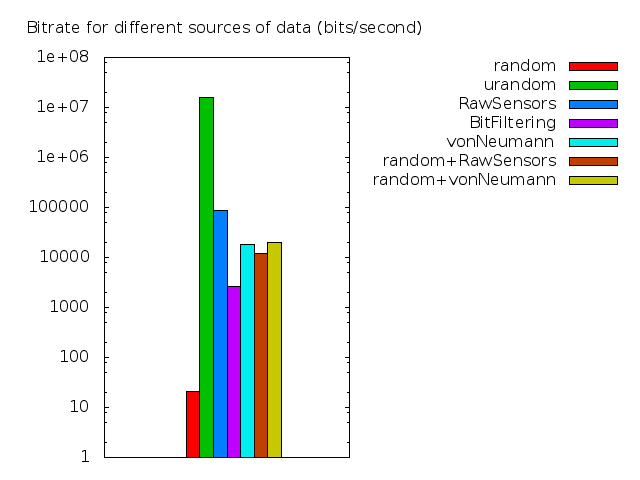
\includegraphics[width=0.5\textwidth]{bitrate.png}
	\caption{Observed bitrate in bits per second.  Note that the y-axis is 
a logarithmic scale.}
	\label{fig:bitrates}
\end{figure}

As shown in the graphs, any form of raw data not mixed into the entropy pool
with other sources of entropy and hashing is not suitable for use as a source
of random bits.  While the bitrates from the raw sensor data (accelerometer
and gyroscope data combined) are relatively high, these bits fail most of the
NIST tests.  With bit filtering, the proportion of tests that passed is higher
than for the raw data, but overall the data does not prove to be statistically
sound.  Data extracted using von-Neumann whitening is similarly characterized -
a slightly larger proportion of tests on the data passed, but overall the data
fails the test suite.  When data is run through the entropy pool, however, the
situation improves.  The raw accelerometer and gyroscope data being fed to the
pool is sufficiently dispersed (through hashing and mixing with other random
sources) so that it becomes much more uniformly distributed; there is no
reason to apply bit filtering to data because of this.  As expected, the
von-Neumann whitened data processed in the entropy pool is statistically
uniform, passing most of the tests in the testsuite.  These results demonstrate
the strong statistical properties of mixing many independent sources using hash
functions.  Finally it is interesting to note that both the random device and
urandom device pass most of the tests.  This is to be expected, as both these
devices are designed to provide statistically uniform bits.  However, as
previously mentioned, random is a true random number source while urandom is
only a pseudo-random source.  This means more analysis is required to prove
whether data is actually random, or merely statistically uniform.  However the
NIST testsuite shows that data obtained from sensors can be used as a form of
entropy.

The bitrates for different devices indicate some interesting properties.  As
expected, the random device was slower than any other device.  However, the
obtained bitrate was much slower than expected; a bitrate of ~20 bits/second
becomes a bottleneck for any application that requires true random numbers.  It
should be noted that this rate should increase when the phone is in use (more
data is being generated, hence a larger amount of entropy).  As also expected,
the pseudo-random device had a bitrate orders of magnitude larger than any other
device.  This is because the device is CPU-bound - it does not need to wait for
any events for data to be generated.  The bitrates of the remaining devices are
intuitive; utilizing raw data from the gyroscope and accelerometer as soon as it
becomes available is faster than performing any sort of post-processing.  Bit
filtering and von-Neumann whitening are slower than simply using raw data, but
are faster than the other devices because they do not incur the overhead of
stirring the data into the entropy pool.  Finally, the devices that utilize the
entropy pool are the slowest (besides the random device, which is orders of
magnitude slower).  Interestingly, the bitrate for von-Neumann whitened data run
through the entropy pool is higher than the bitrate of the raw data run through
the entropy pool - this highlights the indeterministic nature of the entropy
pool.  While this graph indicates a hierarchy of bitrates, many of these devices
provide data that is unacceptable for use in cryptographic applications.  For
example, even though the raw accelerometer and gyroscope data can be provided
at a higher bitrate than several of the other sources, the bits obtained fail
almost every single statistical test.  This stresses the importance of finding a
balance between the quantity and quality of random data obtained from these
devices, possibly based on the needs of the application.


\section{Future Work}
In this paper we present analysis for two sensors on an Android smartphone,
the accelerometer and gyroscope.  However, smartphones are becoming
increasingly diverse in terms of capabilities; many newer devices include
near-field communications, GPS, magnetometers, etc.  Additionally, phones
contain cameras, microphones and touchscreens, all of which have been studied
as sources of random bits.  These sensors and devices could potentially be
leveraged in concert to increase the diversity of data sources and potentially
increase the entropy in the produced data.

Another aspect of these devices to explore is the impact of utilizing several
of these sources at different sampling rates with regards to battery life.
Because these devices already require low power processors and strive to be
as energy efficient as possible, activating and utilizing these devices may
prove this approach infeasible for real-world usage.  Analysis of power usage
would require careful control and handling of variability in battery life.

One feature of the Android ecosystem, which is simultaneously an advantage and
a disadvantage, is the variability in phone designs.  While we have evaluated
one set of sensors on a particular model of phone, there are
innumerable designs for which the data obtained from the sensors varies widely.
Initial testing of several newer models of phones shows that raw data from the
accelerometer and gyroscope may provide higher-quality random bits than
the values obtained from the Nexus S.  Evaluating a wide range of these devices
could provide better insight into whether using these devices for true random
number generation is a viable means for augmenting the sources of entropy for
the Linux entropy pool.

Finally, further investigating different types of post processing may also provide a
means for obtaining higher quality bits from the devices.  While we have
presented several basic forms of post processing (bit filtering and Von Neumann
whitening), many authors have published work in the field of randomness
extraction.  Barak et. al. propose a mathematical model based on the influence
an attacker may have over the source of random data, and an approach to
constructing a randomness extraction function which is guaranteed to provide
good random bits \cite{true_rng_changing_environments}.  Additionally, Barak
et. al. propose a method for combining data from independent sources to
provide higher quality random bits \cite{independent_sources}.  Both of these
approaches could be leveraged to increase the quality of the data obtained
from the sensors.



\section{Conclusion}

% An example of a floating figure using the graphicx package.
% Note that \label must occur AFTER (or within) \caption.
% For figures, \caption should occur after the \includegraphics.
% Note that IEEEtran v1.7 and later has special internal code that
% is designed to preserve the operation of \label within \caption
% even when the captionsoff option is in effect. However, because
% of issues like this, it may be the safest practice to put all your
% \label just after \caption rather than within \caption{}.
%
% Reminder: the "draftcls" or "draftclsnofoot", not "draft", class
% option should be used if it is desired that the figures are to be
% displayed while in draft mode.
%
%\begin{figure}[!t]
%\centering
%\includegraphics[width=2.5in]{myfigure}
% where an .eps filename suffix will be assumed under latex, 
% and a .pdf suffix will be assumed for pdflatex; or what has been declared
% via \DeclareGraphicsExtensions.
%\caption{Simulation Results}
%\label{fig_sim}
%\end{figure}

% Note that IEEE typically puts floats only at the top, even when this
% results in a large percentage of a column being occupied by floats.


% An example of a double column floating figure using two subfigures.
% (The subfig.sty package must be loaded for this to work.)
% The subfigure \label commands are set within each subfloat command, the
% \label for the overall figure must come after \caption.
% \hfil must be used as a separator to get equal spacing.
% The subfigure.sty package works much the same way, except \subfigure is
% used instead of \subfloat.
%
%\begin{figure*}[!t]
%\centerline{\subfloat[Case I]\includegraphics[width=2.5in]{subfigcase1}%
%\label{fig_first_case}}
%\hfil
%\subfloat[Case II]{\includegraphics[width=2.5in]{subfigcase2}%
%\label{fig_second_case}}}
%\caption{Simulation results}
%\label{fig_sim}
%\end{figure*}
%
% Note that often IEEE papers with subfigures do not employ subfigure
% captions (using the optional argument to \subfloat), but instead will
% reference/describe all of them (a), (b), etc., within the main caption.


% An example of a floating table. Note that, for IEEE style tables, the 
% \caption command should come BEFORE the table. Table text will default to
% \footnotesize as IEEE normally uses this smaller font for tables.
% The \label must come after \caption as always.
%
%\begin{table}[!t]
%% increase table row spacing, adjust to taste
%\renewcommand{\arraystretch}{1.3}
% if using array.sty, it might be a good idea to tweak the value of
% \extrarowheight as needed to properly center the text within the cells
%\caption{An Example of a Table}
%\label{table_example}
%\centering
%% Some packages, such as MDW tools, offer better commands for making tables
%% than the plain LaTeX2e tabular which is used here.
%\begin{tabular}{|c||c|}
%\hline
%One & Two\\
%\hline
%Three & Four\\
%\hline
%\end{tabular}
%\end{table}


% Note that IEEE does not put floats in the very first column - or typically
% anywhere on the first page for that matter. Also, in-text middle ("here")
% positioning is not used. Most IEEE journals/conferences use top floats
% exclusively. Note that, LaTeX2e, unlike IEEE journals/conferences, places
% footnotes above bottom floats. This can be corrected via the \fnbelowfloat
% command of the stfloats package.



%\section{Conclusion}
%The conclusion goes here.




% conference papers do not normally have an appendix


% use section* for acknowledgement
%\section*{Acknowledgment}


%The authors would like to thank...

% trigger a \newpage just before the given reference
% number - used to balance the columns on the last page
% adjust value as needed - may need to be readjusted if
% the document is modified later
%\IEEEtriggeratref{8}
% The "triggered" command can be changed if desired:
%\IEEEtriggercmd{\enlargethispage{-5in}}

% references section

% can use a bibliography generated by BibTeX as a .bbl file
% BibTeX documentation can be easily obtained at:
% http://www.ctan.org/tex-archive/biblio/bibtex/contrib/doc/
% The IEEEtran BibTeX style support page is at:
% http://www.michaelshell.org/tex/ieeetran/bibtex/
%\bibliographystyle{IEEEtran}
% argument is your BibTeX string definitions and bibliography database(s)
%\bibliography{IEEEabrv,../bib/paper}
%
% <OR> manually copy in the resultant .bbl file
% set second argument of \begin to the number of references
% (used to reserve space for the reference number labels box)


\bibliographystyle{plain}
\bibliography{final_report}

\appendix
\onecolumn
\begin{figure}[htbp]
    \centering
	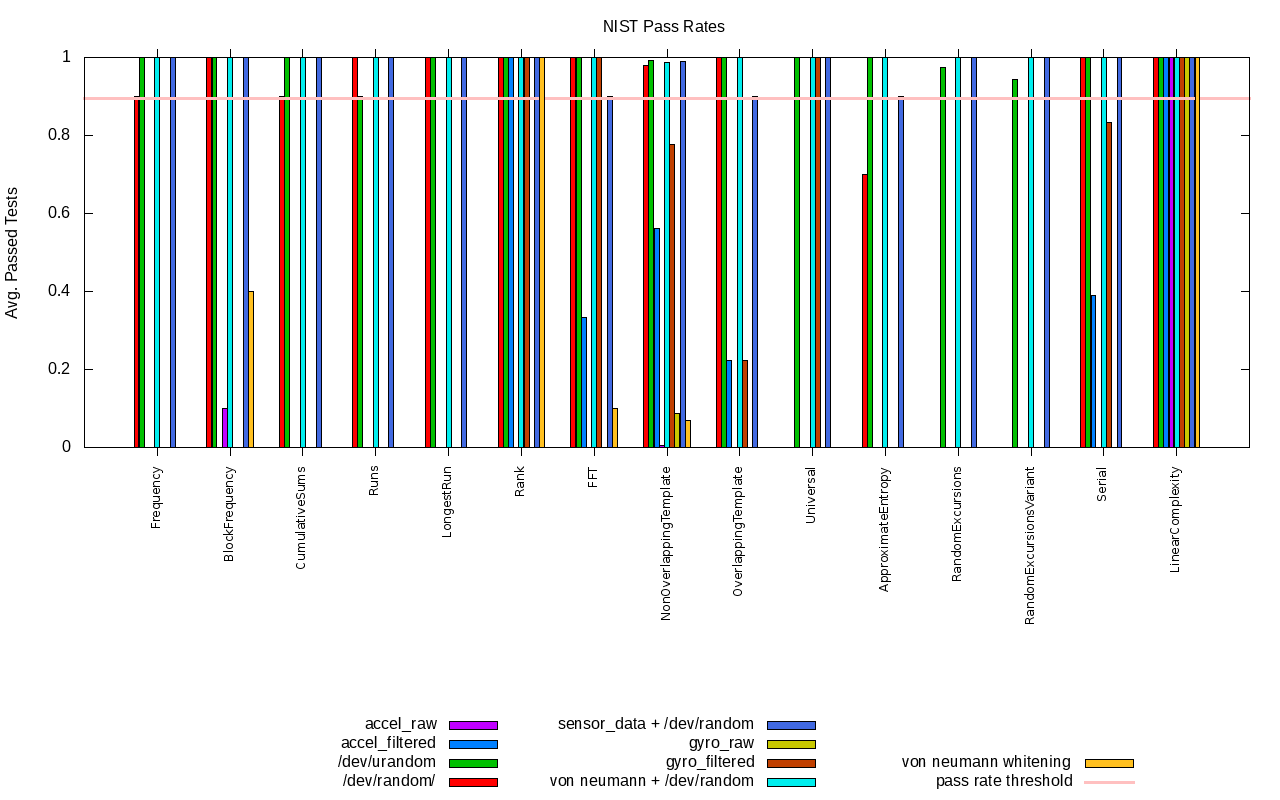
\includegraphics[angle=270,scale=0.5]{nist_results.png}
	\caption{}
	\label{fig:nist_results}
\end{figure}
\twocolumn

% Appendx
\appendix
\section{Graphs}

\begin{figure}[h]
	\centering
	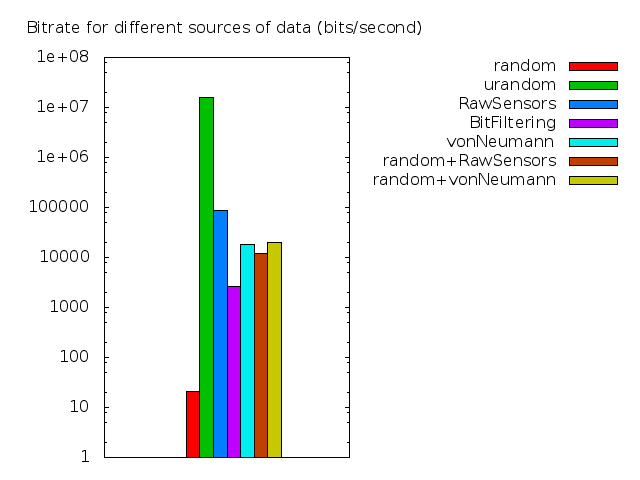
\includegraphics[width=0.5\textwidth]{bitrate.png}
	\caption{Observed bitrate in bits per second.  Note that the y-axis is 
a logarithmic scale.}
	\label{fig:bitrates}
\end{figure}

% that's all folks



\end{document}


